%
% $File: report.tex
% $Date: Fri Dec 27 21:19:54 2013 +0800
%

\documentclass{article}
\usepackage{fontspec}
\usepackage{zhspacing,url,amsmath,amssymb,verbatim}
\usepackage{pdfpages}
\zhspacing
\usepackage{listings}
\usepackage[hyperfootnotes=false,colorlinks,linkcolor=blue,anchorcolor=blue,citecolor=blue]{hyperref}
\usepackage[backend=biber]{biblatex}
\usepackage{graphicx}
\usepackage{minted}
\usepackage{subfigure}
\usepackage{indentfirst}
\usepackage{cases}
\usepackage{environ}
\usepackage{array}
\usepackage[top=1in, bottom=1in, left=1.25in, right=1.25in]{geometry}
\usepackage{caption}
%\usepackage{tikz}
%\usepackage{dot2texi}

% $File: mint-defs.tex
% $Date: Sun Nov 17 23:37:24 2013 +0800
% $Author: Xinyu Zhou <zxytim@gmail.com>

\newcommand{\inputmintedConfigured}[3][]{\inputminted[fontsize=\footnotesize,
	label=#3,linenos,frame=lines,framesep=0.8em,tabsize=4,#1]{#2}{#3}}

\newcommand{\txtsrc}[2][]{\inputmintedConfigured[#1]{text}{#2}}
\newcommand{\txtsrcpart}[4][]{\txtsrc[firstline=#3,firstnumber=#3,lastline=#4,#1]{#2}}

\newcommand{\cppsrc}[2][]{\inputmintedConfigured[#1]{cpp}{#2}}
\newcommand{\cppsrcpart}[4][]{\cppsrc[firstline=#3,firstnumber=#3,lastline=#4,#1]{#2}}

\newcommand{\javasrc}[2][]{\inputmintedConfigured[#1]{java}{#2}}
\newcommand{\javasrcpart}[4][]{\javasrc[firstline=#3,firstnumber=#3,lastline=#4,#1]{#2}}

\newcommand{\matlabsrc}[2][]{\inputmintedConfigured[#1]{matlab}{#2}}
\newcommand{\matlabsrcpart}[4][]{\matlabsrc[firstline=#3,firstnumber=#3,lastline=#4,#1]{#2}}

\newcommand{\pysrc}[2][]{\inputmintedConfigured[#1]{matlab}{#2}}
\newcommand{\pysrcpart}[4][]{\matlabsrc[firstline=#3,firstnumber=#3,lastline=#4,#1]{#2}}

%\usepackage[T1]{fontenc}
\usepackage{lmodern}
\usepackage{amssymb,amsmath}
\usepackage{ifxetex,ifluatex}
\usepackage{fixltx2e} % provides \textsubscript
% use upquote if available, for straight quotes in verbatim environments
\IfFileExists{upquote.sty}{\usepackage{upquote}}{}
\ifnum 0\ifxetex 1\fi\ifluatex 1\fi=0 % if pdftex
  \usepackage[utf8]{inputenc}
\else % if luatex or xelatex
  \usepackage{fontspec}
  % commented by Xinyu Zhou
  \ifxetex
    \usepackage{xltxtra,xunicode}
  \fi
  \defaultfontfeatures{Mapping=tex-text,Scale=MatchLowercase}
  \newcommand{\euro}{€}
\fi
% use microtype if available
\IfFileExists{microtype.sty}{\usepackage{microtype}}{}
\usepackage{color}
\usepackage{fancyvrb}
\newcommand{\VerbBar}{|}
\DefineShortVerb[commandchars=\\\{\}]{\|}
\DefineVerbatimEnvironment{Highlighting}{Verbatim}{commandchars=\\\{\}}
% Add ',fontsize=\small' for more characters per line
\newenvironment{Shaded}{}{}
\newcommand{\KeywordTok}[1]{\textcolor[rgb]{0.00,0.44,0.13}{\textbf{{#1}}}}
\newcommand{\DataTypeTok}[1]{\textcolor[rgb]{0.56,0.13,0.00}{{#1}}}
\newcommand{\DecValTok}[1]{\textcolor[rgb]{0.25,0.63,0.44}{{#1}}}
\newcommand{\BaseNTok}[1]{\textcolor[rgb]{0.25,0.63,0.44}{{#1}}}
\newcommand{\FloatTok}[1]{\textcolor[rgb]{0.25,0.63,0.44}{{#1}}}
\newcommand{\CharTok}[1]{\textcolor[rgb]{0.25,0.44,0.63}{{#1}}}
\newcommand{\StringTok}[1]{\textcolor[rgb]{0.25,0.44,0.63}{{#1}}}
\newcommand{\CommentTok}[1]{\textcolor[rgb]{0.38,0.63,0.69}{\textit{{#1}}}}
\newcommand{\OtherTok}[1]{\textcolor[rgb]{0.00,0.44,0.13}{{#1}}}
\newcommand{\AlertTok}[1]{\textcolor[rgb]{1.00,0.00,0.00}{\textbf{{#1}}}}
\newcommand{\FunctionTok}[1]{\textcolor[rgb]{0.02,0.16,0.49}{{#1}}}
\newcommand{\RegionMarkerTok}[1]{{#1}}
\newcommand{\ErrorTok}[1]{\textcolor[rgb]{1.00,0.00,0.00}{\textbf{{#1}}}}
\newcommand{\NormalTok}[1]{{#1}}
% \ifxetex
%   \usepackage[setpagesize=false, % page size defined by xetex
%               unicode=false, % unicode breaks when used with xetex
%               xetex]{hyperref}
% \else
%   \usepackage[unicode=true]{hyperref}
% \fi
\hypersetup{breaklinks=true,
            bookmarks=true,
            pdfauthor={},
            pdftitle={},
            colorlinks=true,
            urlcolor=blue,
            %linkcolor=magenta,
            pdfborder={0 0 0}}
%\urlstyle{same}  % don't use monospace font for urls
\setlength{\parindent}{0pt}
\setlength{\parskip}{6pt plus 2pt minus 1pt}
\setlength{\emergencystretch}{3em}  % prevent overfull lines
%\setcounter{secnumdepth}{0}



\newcommand{\figref}[1]{\hyperref[fig:#1]{Figure.\ref*{fig:#1}}}
\newcommand{\tableref}[1]{\hyperref[table:#1]{Table.\ref*{table:#1}}}
\newcommand{\centerize}[1]{\begin{center} #1 \end{center}}
\newcommand{\secref}[1]{\hyperref[sec:#1]{Section.\ref*{sec:#1}}}
\newcommand{\appref}[1]{\hyperref[app:#1]{App.\ref*{app:#1}}}


\newcommand{\cmd}[1]{{\it #1}}
\newcommand{\ccmd}[1]{\centerize{\cmd{#1}}}

\title{Digital Signal Processing: Speaker Recognition \\ Final Report \\ Concise Version}
\author{Xinyu Zhou, Yuxin Wu, and Tiezheng Li\\ Tsinghua University}
\date{}

\bibliography{refs.bib}
\begin{document}

\fontsize{11pt}{1.4em}
\setlength{\baselineskip}{1.6em}
\maketitle

\section{Dataset}
	The dataset provided by teacher comprised of 102 speaker, in which 60 are
	females and the rest are males, with three different speaking style: Spontaneous,
	Reading and Whisper. A statistic is as follows:
	\begin{table}[!ht]
		\centering
		\begin{tabular}{|c|c|c|c|}
			\hline
			& Spontaneous & Reading & Whisper \\\hline
			Average Duration & 202s & 205s & 221s \\\hline
			Female Average Duration & 205s & 202s & 217s \\\hline
			Male Average Duration & 200s & 203s & 223s \\\hline
		\end{tabular}
	\end{table}

\section{Approach}

Based on weeks of literature reviewing and testing,
we have designed our overall approach to this task as followed:

\begin{enumerate}
    \item Energy-Based VAD

      Input audio signals are very likely to contain significantly large ratio of blank signals.
      VAD (Voice Activity Detector)
      is a preprocessing technique to filter out the blank period.
      The most common approach toward this goal is to use energy-based feature of signals.

      \item Cepstrum-Based Features

        Research showed that cepstrum-based features are more discrimitive in the task of speech and speaker recognition/verification.
        We decide to apply common cepstrum features extraction routine, such as MFCC (Mel-frequency Cepstrum Coefficients), LFCC,
        after the original signals are preprocessed by VAD.

       The basic procedure of MFCC is shown below, and the details about
       extracting MFCC is already been explained in the previous reports.
       The output of this step, is a sequence of fixed-dimension vectors, which will be used later in model training.

      \begin{figure}[H]
        \centering
        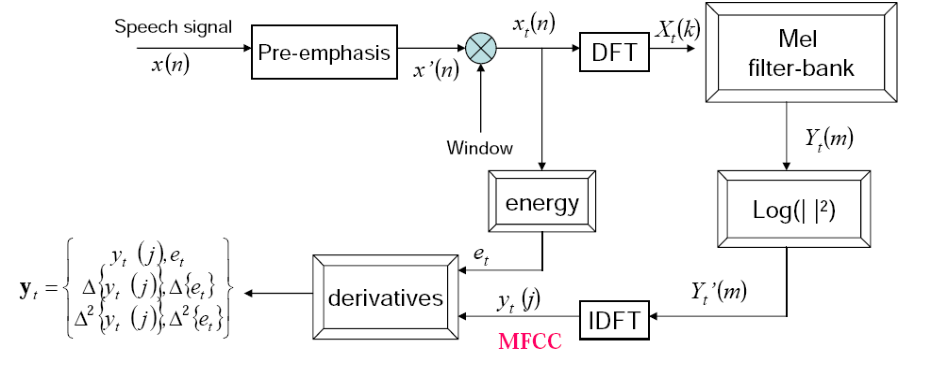
\includegraphics[width=\textwidth]{res/MFCC.png}
      \end{figure}

    \item GMM and UBM Model

      Since the feature vectors of a speaker tend to cluster into \textbf{several} groups
      in the feature space,
      the model of a specific speaker can be well described by using GMM (Gaussian Mixture Model).
      Moreover, for different speakers, the components of their individual GMMs
      will also have similar distributions, which discriminate different syllables.
      Therefore, an UBM (Universal Background Model) can be first trained for all speakers,
      and then we can get adapted GMMs which fit this task better.

      \begin{figure}[H]
        \centering
        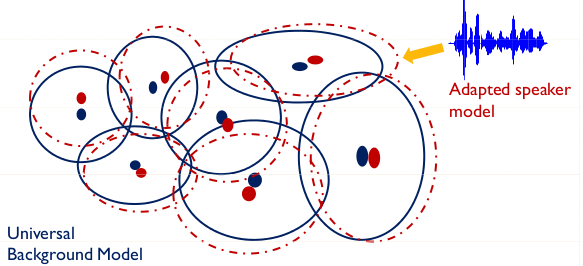
\includegraphics[width=0.7\textwidth]{res/ubm.png}
      \end{figure}

      \item JFA
        GMM-based model can describe the clusterred distribution, but it fails to account for
        different types of variability in each clusterred group.
        However, we only need inter-speaker variability to be modeled,
		but not channel or noise variability. Join Factor Analysis can convey
		such information.

  \end{enumerate}


\section{Result}
\label{sec:result}
We have tested our method on a corpus provided by teacher Xu. For detailed
description of the corpus, please see former report.

All the tests are conducted serval times (depending on computation cost,
vary from 5 to 20) with random selected training and testing speakers.
The average over these tests are considered as the final
result.

\subsection{Efficiency Test of our GMM}
We have extensively examined the efficiency of our implementation of GMM
compared to scikit-learn version. Test is conducted using real MFCC data with
13 dimensions. We consider the scenario when training a UBM with 256 mixtures.
We examine the time used for ten iteration.  For comparable results, we diabled
the K-means initialization process of both scikit-learn GMM implementation and
ours.  Time used for ten iterations under different data size and concurrency
is recorded.

\begin{figure}[!ht]
	\begin{minipage}{0.48\linewidth}
		\centering
		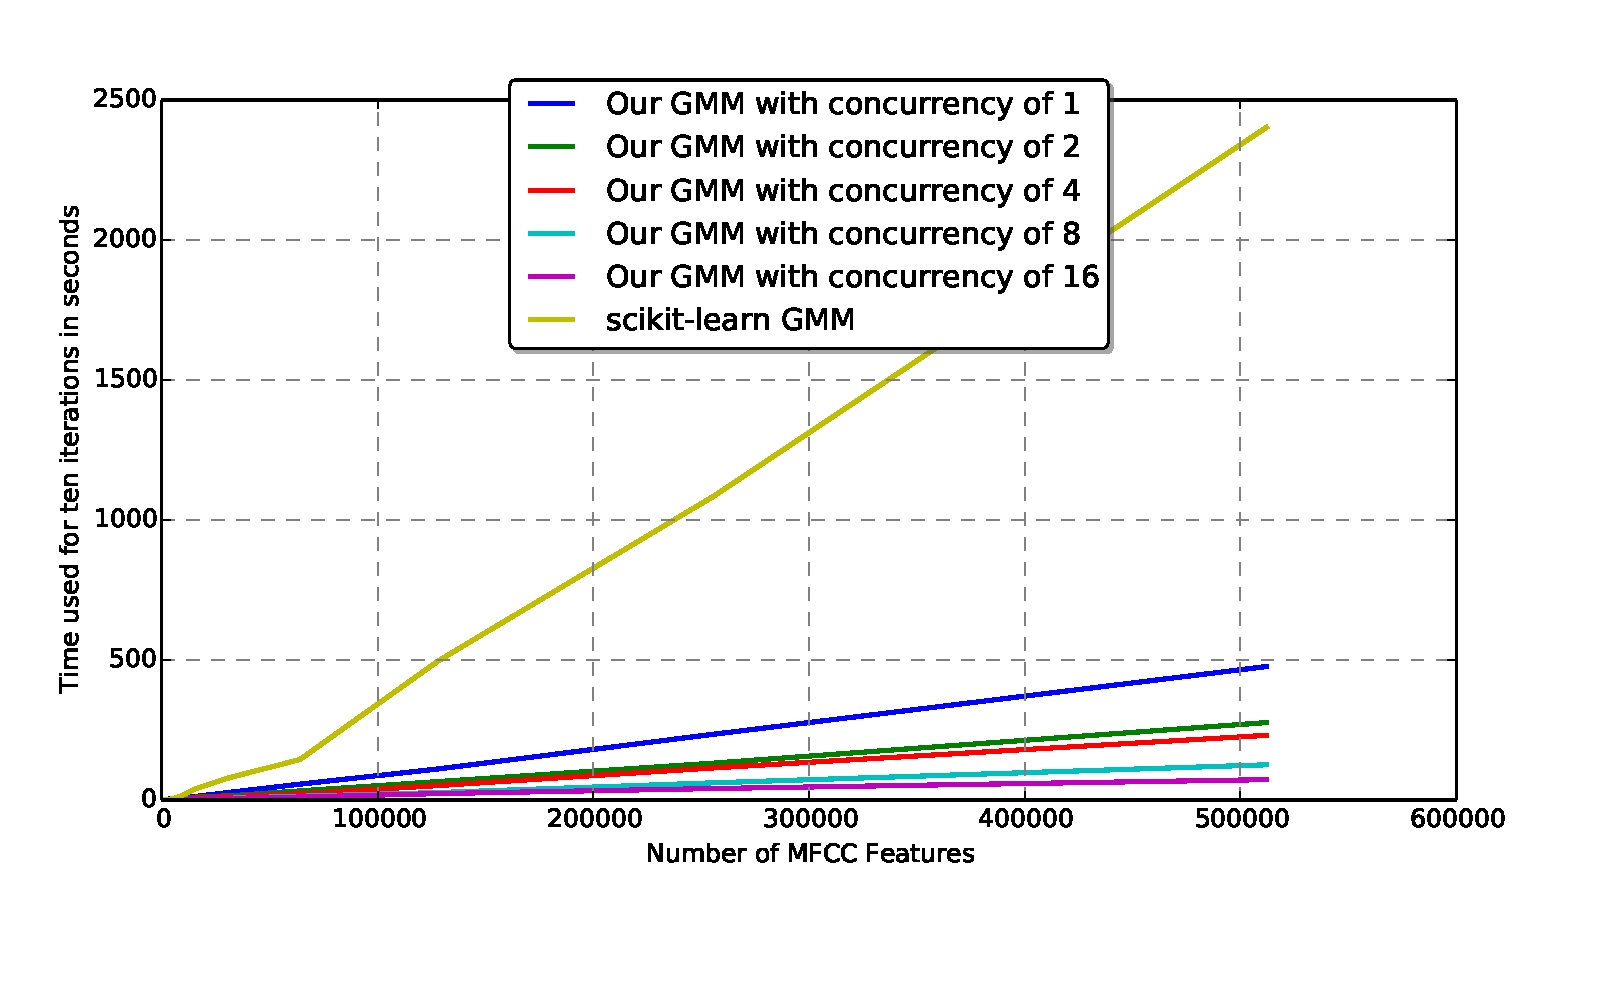
\includegraphics[width=\linewidth]{res/time-comp.pdf}
		\caption{Comparison on efficiency\label{fig:gmm_efficiency}}
	\end{minipage}
	\hfill
	\begin{minipage}{0.48\linewidth}
		\centering
		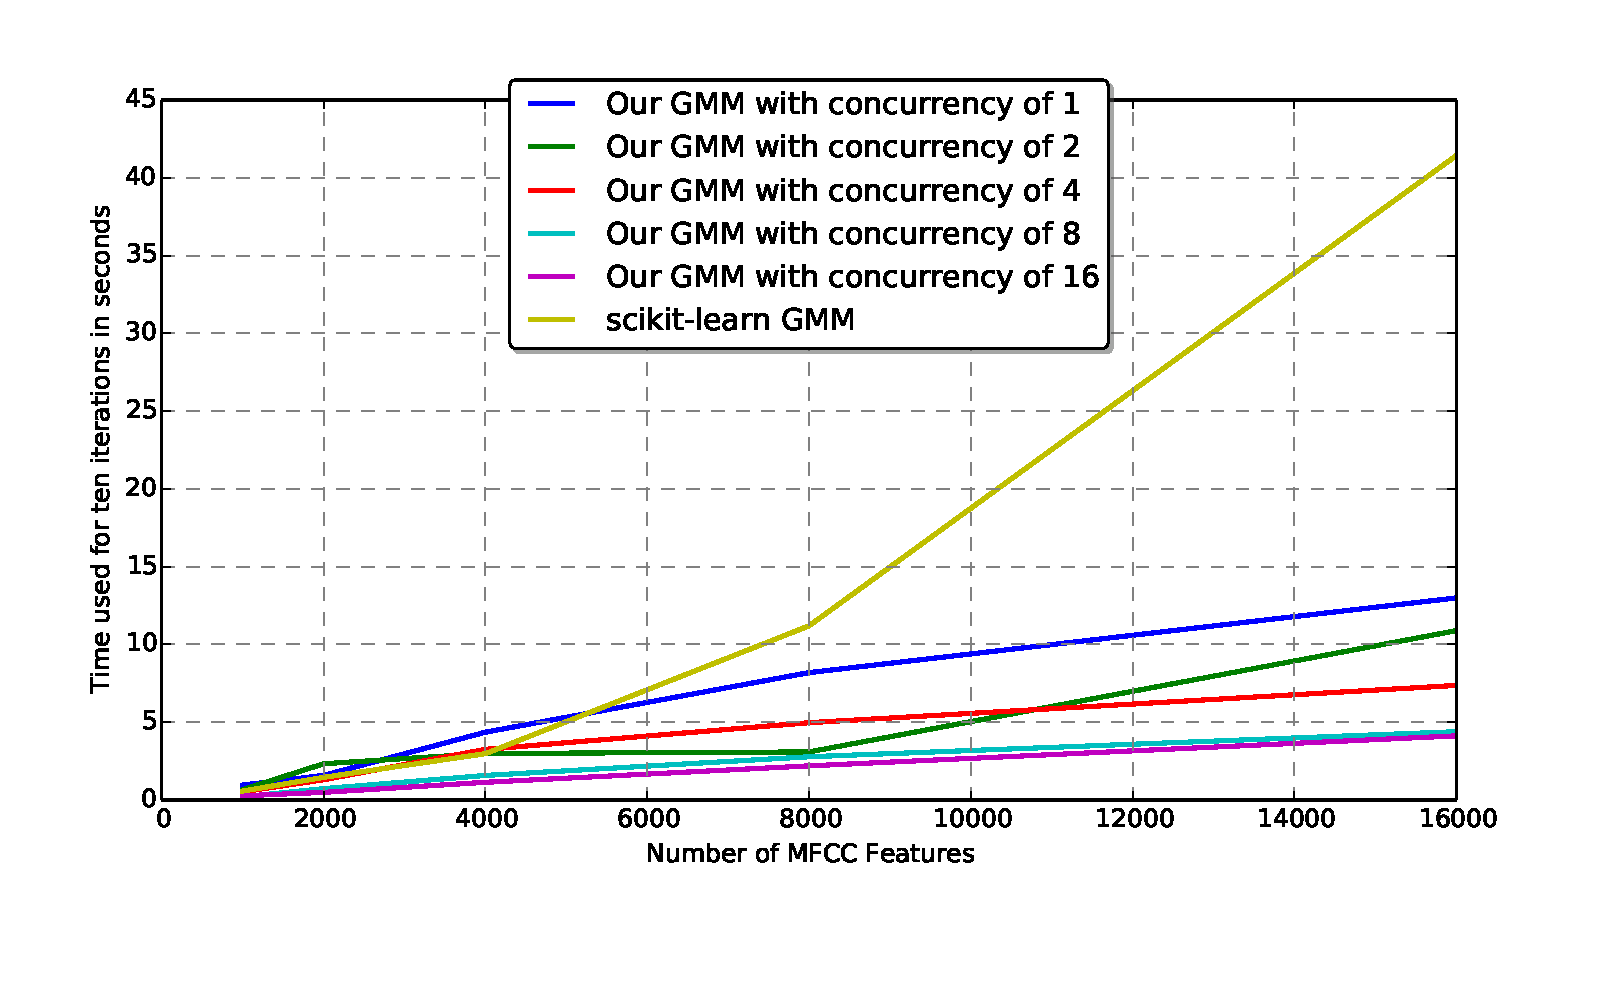
\includegraphics[width=\linewidth]{res/time-comp-small.pdf}
		\caption{Comparison on efficiency when number of MFCC features is small\label{fig:gmm_efficiency_small}}
	\end{minipage}
\end{figure}

From \figref{gmm_efficiency}, we can immediately infer that our method
is much-much more efficient than the widely used version of GMM provided
by scikit-learn when the data size grows sufficiently large.

We shall analyze in two aspect:
\begin{itemize}
	\item No concurrency
		\begin{itemize}
			\item When the number of MFCC features is below 6000, which is a typical
				number of features generated by 60 seconds utterances (1ms frame shift),
				our method is slightly slower; but this is trivial since
				1 minute utterance is too small.
			\item When the number of MFCC features grows sufficiently large, our method
				shows great improvement. When training 512,000 features, our method
				is 5 times faster than comparing method.
		\end{itemize}
	\item With concurrency \\
		Our method shows considerable concurrency scalability that the running time
		is approximately lineary to the number of cores using.

		When using 8-cores, our method is \textbf{$19$ times} faster than comparing
		method.
\end{itemize}


\subsection{Effect Of Number Of Mixtures}
We examined our GMM compared to GMM from scikit-learn.
Test is conducted on 30-speaker corpus, 30 seconds training utterance
and 100 random sampled 5 seconds test utterance for each speaker.

As \figref{mixture} illustrates, when number of mixtures is small,
our GMM outperforms scikit-learn version by $10\%$, which indicates our
GMM models the distribution more accurately. The maximum accuracy
happens when the number of mixtures is around 32, reaching $0.965$. As
the number of mixtures increases, the decrease in accuracy

\begin{figure}
	\centering
	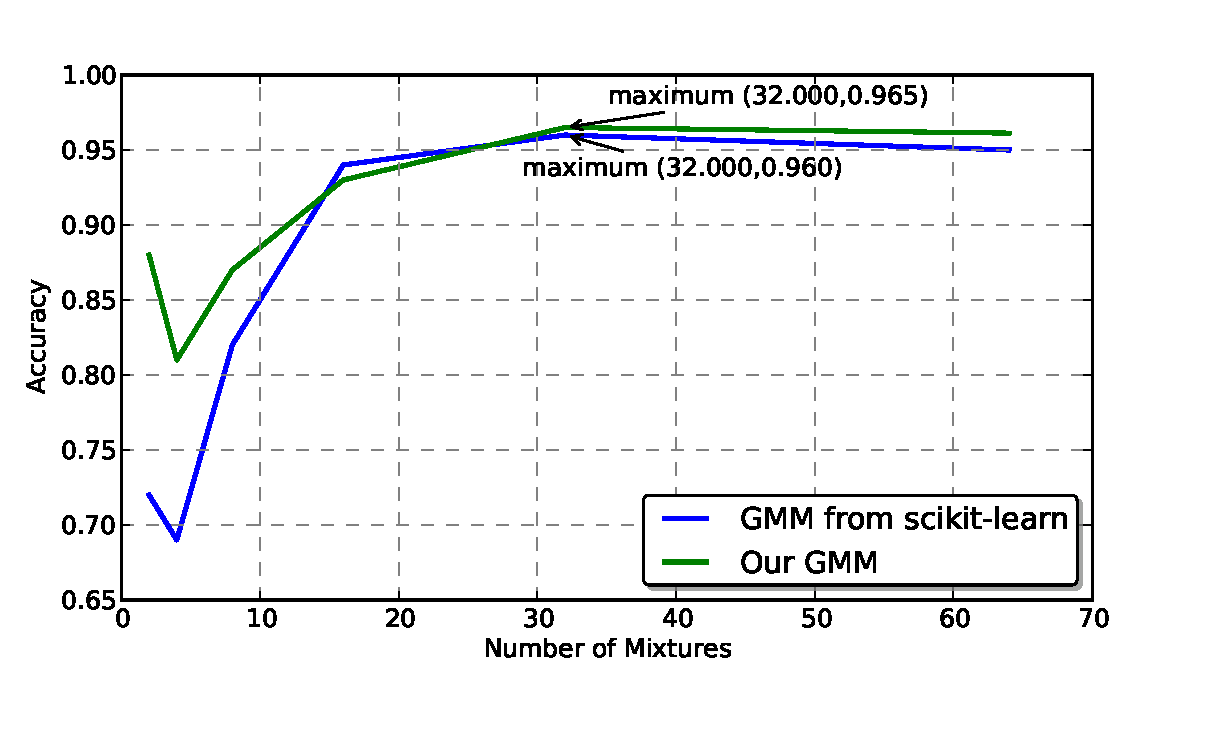
\includegraphics[width=\linewidth]{res/mixture-both.pdf}
	\caption{Accuracy curve on different number of mixtures\label{fig:mixture}}
\end{figure}

\section{Effect On Number Of Speakers}
An apparent trade-off in speaker recognition task is the number of speakers
enrolled and the accuracy of recognizing a person. We've conducted experiments
examining the effect of number of speakers enrolled on the performance of the
system.

The configurations of the test is as followed:
\begin{itemize}
	\item Number of mixtures is set to 32, the optimal number we found previously
	\item GMM from scikit-learn, compared to our GMM.
	\item 30s training utterance and 5s test utterance
	\item 100 sampled test utterance for each user
\end{itemize}


\begin{figure}[!ht]
	\centering
	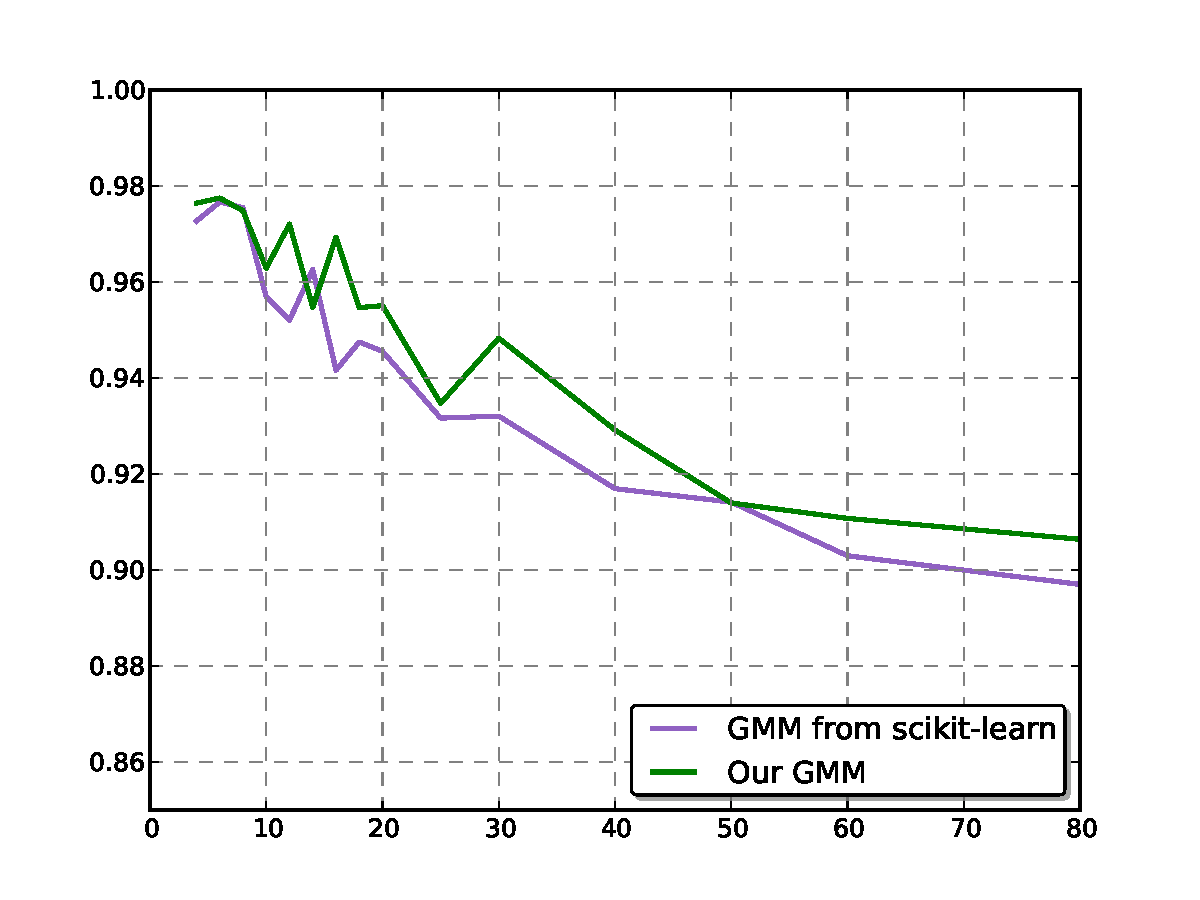
\includegraphics[width=\linewidth]{res/nperson.pdf}
	\caption{Accuracy curve on different number of speakers enrolled\label{fig:nspk_enrolled}}
\end{figure}

Scrunitizing \figref{nspk_enrolled} we would see that, our GMM performs better than
scikit GMM in general. When number of speakers is small, due to the the random
selection, the variance of the tests is significantly high, as we can see from the curve fluctuants.
When number of speakers increases, it is clear that the
accuracy of our GMM is above scikit version. As the more speaker, the more
difficult the recognition task will be, this result suggests that our
optimization on GMM takes effect.



\section{GUI}
	This section describes the design of Graphic User Interface to accomodate our system.
\subsection{Functional Requirements}
	The GUI consists of following functions:
	\begin{itemize}
		\item \textbf{Enrollment of speaker} \\
			A new user can be dynamically add to this system.\
			when enrollment starts, the user is prompted to input
			his identifications, e.g, name, age, sex, a photo would
			be better, and so on.

			Then he is required to record a piece of utterance.
			An article will be prompted to the user in case he/she
			is introrse to say something, he/she can read the article.

			There are two ways to enroll a user:
			\begin{itemize}
				\item \textbf{Enroll by speaking}
					A progress indicator of enrollment process will be present to user.
					When enough utterance is collected, the user will be given
					message about the success of enrollment.

				\item \textbf{Enroll by pre-recorded voice}
					User can upload a pre-recorded voice of a speaker. The system
					accepts the voice given and the enrollment of a speaker is done.
			\end{itemize}

		\item \textbf{Recognition of a user} \\
			A enrolled user present and record a piece of utterance,
			the system tells who the person is.

		\item \textbf{Conversation Recognition mode} \\
			When the system turn into Conversation Recognition mode,
			it will continuously collect voice data, and determine
			who is speaking right now. If a photo is given in previous
			enrollment process, current speaker's photo will show up
			in screen; otherwise the name will be shown.

		\item \textbf{Verification mode} \\
			A user first claim its identity, then the system required
			the user to record a piece of utterance. The system will
			then display whether the speaker is the speaker that claimed
			or an impostor.

			The availability of this function is still under our investigation.

	\end{itemize}

\subsection{Non-Functional Requirements}
	\begin{itemize}
		\item \textbf{Enrollment Efficiency} \\
			The enrollment procedure involves training GMM or RBM model, which
			is a time consuming process. A continuous flow of user enrollment
			should not be interupted.
		\item \textbf{Platform-Independency} \\
			As we program using Python, our program should run on
			platform that supports Python.
		\item \textbf{Recognition Accuracy} \\
			The performance of the system should be good enough to
			make this system could be carried out in practical use.
	\end{itemize}


\printbibliography

\end{document}

